% !TeX root = ../main.tex
% %%%%%%%%%%%%%%%%%%%%%%%%%%%%%%%%%%%%%%%%%%%%%%%%%%%%%%%%%%%%%%%%%%%%%%%%%%%%%%
% Introduction
\chapter{Introduction}
\label{chap:introduction}

Be it a robot arm in a car assembly line, your vacuum cleaner, or a cat-like robot to carry 
your food in a restaurant, robotics already have a great impact on our current society. 
Due to their broad practicality, the quality of software 
used by robots should be of extreme importance for us.
Robot software as well as the techniques used to test their quality are very 
field-specific and different from the techniques employed in traditional Software Engineering.
Automatic tests are barely used in robotics due to multiple factors:
cost, complexity, hardware integration, among others~\cite{TestRob}.
The goal of this thesis is to overcome the challenges of automated 
testing in robotics, by providing developers with a usable alternative 
that allows detecting bugs with less effort through simulation.


% ------------------------------------------------------------------------------
% Motivation
\section{Motivation}
\label{sec:motivation}

Today, robots are vastly used industrially (medicine, agriculture, etc.) 
or leisurely (contests, personal use, etc.).
The tendency is for robot usage to keep growing at a global level.
Robot tasks tend to be repetitive and rather specific.
Therefore, Robot software also tends to be quite different from conventional software.
The Cyber-Physical systems of robots are non-deterministic and unreliable, 
mainly because robots interact directly with their environment.
A sensor can return imprecise values since the environment itself can be very hard to predict.
As a result, verifying whether a task or movement is correct is hard for a robot to conceive.

\par

Current practices on testing robot software are common among developers, 
including field testing, simulation testing, logs checking, among others.
The common denominator among these is that they require a human to analyze 
the behavior of the robot to determine whether the behavior is correct. 
If there was a tool that could make this decision, automated tests 
could be used more widely in robot systems.
However, that is not the case as automatic tests are hardly used. 
Opening this door would mean an improvement in the 
quality of current and future robot software.


\section{Problem Statement}
\label{sec:problem}

The multiple challenges in robot testing have an influence on planning 
how to test a robot because there are tradeoffs among choices.
While simulation-based tests are a promising approach for automation 
there is still distrust in the precision and validity of the results.
This means that, despite being dangerous and sometimes expensive, 
real-life robot testing is still the main choice.
Both in real-world testing or simulations, 
human supervising will most likely still be necessary.
This is because identifying if a robot fulfills an expected 
behavior is very hard for the robot itself.
For this reason, automatic tests in the robotics field are 
hardly reliable and hard to implement.
The resulting product is a lack of quality in the software 
across projects.
In short, right now in the field is manually costly to identify 
test scenarios and identify if the robot does what we want.


% ------------------------------------------------------------------------------
% Objectives
\section{Objectives}
\label{sec:objectives}

This work has the objective of showing the potential of automatic 
tests in robotics and of simplifying their execution.
With this in mind, we propose a mechanism that monitors a subset of 
the components of the robot during or after tests execution.
These components aren't arbitrary but are defined with the help of a descriptive high-level language.
Not only the components but the test scenario should be described in this language.
With the description of this language, one should be able to detect and 
orchestrate relevant robot components associated with the testing scenario.
The language should allow describing a robot property in a simple and intuitive way.
This language will need to be supported by a compiler. 
The compiler should translate the language to a monitoring mechanism.
In this way, if a robot doesn't follow the properties defined by the 
language, either during execution or a log analysis, the compiler will 
detect an anomaly in the normal behavior of the robot.


%Maybe no image here
%\begin{figure}[h!]
%    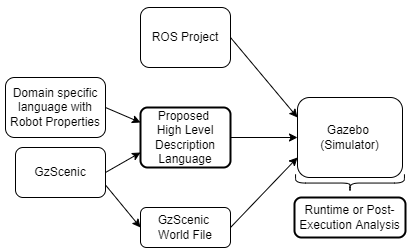
\includegraphics{images/intro_diag.png}
%    \caption{Tool for monitoring robot properties.}
%    \label{fig:intro_objectives}
%\end{figure}

\section{Contributions}
\label{sec:contributions}

The expected contributions of this thesis are below enumerated.

\begin{enumerate}
    \item Definition of a descriptive high-level language to specify robots properties.
    \item Implementation of compiler for the language that can be used for monitoring.
    \item Evaluation of the expressive capability of the solution in real-world examples.
\end{enumerate}

% ------------------------------------------------------------------------------
% Structure of the document
\section{Structure of the document}
\label{sec:structure}

The document is organized as follows:

\begin{itemize}
    \item Section 1...
    \item Section 2...
    \item Section 3...
\end{itemize}

